% Ansatz.tex
\chapter{Eclipse SmartHome}
\label{chap:esh}
In diesem Kapitel wird \textit{Eclipse SmartHome} (ESH) \cite{ESH:home} vorgestellt. Es werden zunächst die grundlegenden Konzepte des Frameworks erläutert. Anschließend wird auf für die Arbeit relevante konkrete Aspekte näher eingegangen.

\section{Überblick}
Eclipse SmartHome positioniert sich als ein Framework, dass als Grundlage für die Entwicklung von konkreten SmartHome Anwendungen dienen soll. Tatsächlich kommt es in vielen bekannten Produkten zum Einsatz, wie z.B. openHAB\cite{openHAB} oder Qivicon\cite{qivicon}.


\subsubsection{Architektur}
Eclipse SmartHome hat eine serviceorientierte Architektur, basierend auf dem Java OSGi Framework\cite{osgibook}. OSGi spezifiziert eine dynamische Softwareplattform, die hardwareunabhängig ist und es ermöglicht, Anwendungen zu modularisieren und zu verwalten. Der Funktionsweise der Kommunikation ist in Abbildung \ref{fig:osgi} veranschaulicht.

\begin{figure}[h]
	\centering
	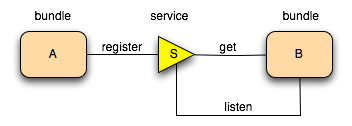
\includegraphics{bilder/osgi}
	\caption{OSGi Komponentenmodell: Kommunikation zwischen Bundles \cite{osgi:whatisit}}
	\label{fig:osgi}
\end{figure}

Im Rahmen des OSGi Frameworks wird das gesamte Programm in verschiedene Softwarekomponenten (Bundles) aufgeteilt. Jede Komponente bietet und bezieht Services. Die angebotenen Services werden von den entsprechenden Bundles zur Laufzeit im System registriert, wonach andere Bundles, die diese Services beziehen, darüber informiert und ihrerseits gestartet werden können. Ein Bundle wird erst gestartet, wenn alle von ihm benötigten Services im System registriert wurden.\\

Ein derartiger modularer Aufbau erlaubt es verschiedene Bundles nahezu unabhängig von einander zu entwickeln und später einzelne Bundles gegen aktuellere Versionen problemlos auszutauschen. Eclipse SmartHome besteht derzeit aus über 130 solcher untereinander kommunizierender Softwarekomponenten.


\subsubsection{Features}
Trotz der Positionierung als Grundlage für konkrete Smart Home Lösungen anderer Anbieter, verfügt das Framework über den kompletten Service Stack, der in einem SmartHome zum Einsatz kommt. Es existiert ein allgemeines Modellgerüst für die virtuelle Abbildung von realen Geräten. Für einige ausgewählte Geräte ist die Steuerung implementiert. Automatisches Auffinden und Einbinden von Geräten wird begrenzt unterstützt. Eine Rule Engine ist bereits integriert. Schließlich gibt es eine rudimentäre Benutzeroberfläche, die es erlaubt zur Laufzeit Geräte zum System hinzuzufügen und sie zu steuern. ESH hat eine ganze Reihe weiterer Features, wie z.B. Sprachunterstützung, die jedoch im Rahmen dieser Arbeit nicht von Interesse sind. 

Zentrales Prinzip des gesamten Frameworks ist es möglichst generische Schnittstellen zu definieren und exemplarische Implementierungen anzubieten, die die beabsichtigte Funktionsweise veranschaulichen. \\

Im Folgenden werden die verschiedenen Aspekte von ESH, die für die Arbeit relevant sind, erläutert.

\section{Modell}
Die virtuelle Abbildung der realen Geräte im System veranschaulicht Abbildung \ref{fig:esh_model}. Der generische Aufbau ermöglicht die Einbindung von sehr unterschiedlichen Funktionalitäten.  Dies wurde durch die Verteilung der Logik auf mehrere Komponenten realisiert. Die zentralen Elemente sind Things, Channels, Items und Links. 

\begin{figure}[h]
	\centering
	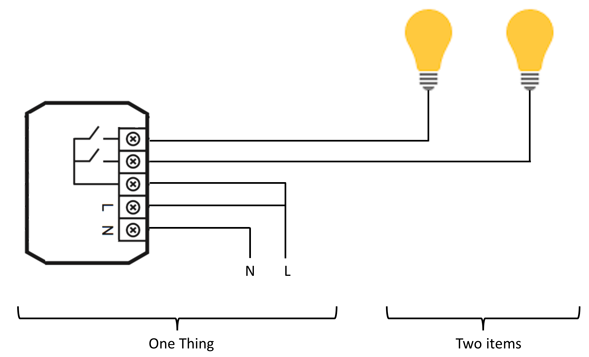
\includegraphics[width=\textwidth]{bilder/esh_model}
	\caption{Architektur von \textit{Things} und \textit{Items} in ESH \cite{ESH:home}}
	\label{fig:esh_model}
\end{figure}

\subsubsection{Things}
Things repräsentieren Entitäten, die zum System hinzugefügt werden können. In der Regel handelt es sich hierbei um verschiedene intelligente Geräte, wie beispielsweise eine \textit{Hue} Lampe oder eine Wetterstation. Derartige Geräte bieten eine oder mehrere Funktionalitäten über Channels an.

Things, die als Brücke zu anderen intelligenten Geräten dienen, werden als Bridges bezeichnet (z.B. \textit{Hue} Bridge);

\subsubsection{Channels}
Ein Channel stellt eine bestimmte Funktionalität eines Things dar. Things können eine beliebige Anzahl von Channels anbieten. Beispielsweise kann eine Hue Lampe einen einzigen \glqq Licht\grqq -Channel anbieten, während eine Wetterstation die Channels \glqq Temperatur\grqq , \glqq Druck\grqq{} und \glqq Feuchtigkeit\grqq{} unterstützt.

\subsubsection{Items}
Items repräsentieren konkrete, detaillierte Funktionalitäten eines Things. Beispielsweise kann ein Thing den Channel \glqq Licht\grqq{} unterstützen, wobei es 2 verschiedene Items besitzt, die beide jeweils eine physische Glühbirne verkörpern. Items haben einen Zustand, der im System gespeichert wird und können Commands empfangen.

\subsubsection{Links}
Links verbinden Items mit Things. Jeder Link assoziiert genau einen Channel des Things mit genau einem Item. Erst wenn ein Channel mit mindestens einem Item verbunden ist, gilt er als \glqq aktiviert\grqq{}. Channels und Items können über eine beliebige Anzahl von Links untereinander verbunden werden.


\subsection{Persistenz}
\label{subsec:persistenz}
In Eclipse SmartHome ist eine MapDB\cite{mapDB} bereits integriert. Dabei handelt es sich um eine leichtgewichtige, eingebettete Datenbank, in der alle Things, Items und Rules persistiert werden. Dies ermöglicht es existierende Entitäten auch nach einem Neustart der Anwendung weiter zu verwenden, ohne sie neu anlegen zu müssen. Da in ESH die Anzahl von persistierten Informationen vergleichsweise gering ist, ist diese Datenbank völlig ausreichend.


\section{Automatisierung}
In ESH herrschen eine Reihe von Design Prinzipien, die sich durch das gesamte Framework verfolgen lassen. Vor allem macht sich die Aufteilung in Modell und Controller bemerkbar: Für sämtliche Entitäten werden zunächst Typen deklariert, für welche über \textit{ModuleTypeProvider} zugehörige Handler im System registriert werden. Dadurch wird die klassische Trennung von Datenmodell und Logik realisiert.

\subsection{Rule Engine}
\label{sec:ruleengine}
Teil des Eclipse SmartHome Frameworks ist eine Regelmaschine. Sie hat eine generische Struktur, die es erlaubt Szenarien zu definieren, die über das typische ECA-Modell hinausgehen. Durch eine Zusammenarbeit von Auslösern (Trigger), Bedingungen (Conditions) und Befehlen (Actions) wird die Automatisierung von Things ermöglicht. Trigger, Conditions und Actions werden in ESH auch als Module bezeichnet.


\subsubsection{Trigger}
Durch Trigger wird die Ausführung einer Regel angestoßen. Die Logik dahinter ist absolut frei implementierbar - der bekannte Aufbau, dass ein hineinkommendes Event den Trigger auslöst, ist nur eine Möglichkeit unter vielen. Dies wird ermöglicht, indem das Auslösen von Triggern von der Regelmaschine los gekoppelt und in einem dedizierten Trigger-Handler behandelt wird. \\

Der Handler erhält nach der Instanziierung einen Callback zur Rule Engine vom System. Über diesen Callback teilt er der Regelmaschine mit, wann immer die Ausführung einer Regel angestoßen werden soll. Wann dies geschieht, muss vom Handler selbst entschieden werden, die Rule Engine hat hierauf keinerlei Einfluss. Beispielsweise, falls der Trigger klassischerweise bei einem Event feuern sollte, müsste der Handler sich als \textit{EventSubscriber} im System registrieren und auf das Event entsprechend reagieren. Alternativ kann an dieser Stelle auch beliebige andere Logik zum Einsatz kommen.\\

Trigger-Handler werden für Instanzen von Triggern über \textit{ModuleTypeProvider} bereitgestellt. Solche Provider sind dafür verantwortlich für bestimmte Modul-IDs zugehörige Handler zur Verfügung zu stellen. Jedes Mal, wenn eine Instanz eines Moduls im System erzeugt wird, wird unter den registrierten Providern nach einem passenden gesucht, der für die ID des Moduls einen Handler generieren kann. Falls kein entsprechender Handler instanziiert werden kann, bleibt das Modul tot im System liegen und sämtliche damit gekoppelte Funktionalitäten fallen aus. Beispielsweise würde eine Rule, die einen Trigger enthält, für den kein korrespondierender Handler erzeugt werden kann, im System als \glqq nicht initialisiert\grqq{} untätig bleiben.

\subsubsection{Kontext}
\label{subsubsec:kontext}
Während der Ausführung einer Rule ist ein Kontext gegeben, der stets von den Triggern über die Conditions an die Actions weitergereicht wird, was es ermöglicht komplexe Logik einzubauen. Alle Komponenten der Regel erhalten ihn bei der Ausführung übergeben und können ihn mit Informationen füllen. Beispielsweise kann das auslösende Event im Kontext gespeichert werden, sodass die darauffolgende Condition aufgrund derer eine Entscheidung treffen kann, ob die Actions tatsächlich ausgeführt werden sollen. Eine Action könnte anhand des Kontextes identifizieren, auf welchen Wert ein Item geschaltet wird.

\subsubsection{Conditions}
Conditions sind analog zu Triggern aufgebaut. Sie agieren als Filter, indem sie festlegen, ob eine Regel, die durch einen Trigger angestoßen wurde, die zugehörigen Actions in Wirklichkeit ausführt. Bedingungen haben ebenfalls Handler, die den Kontext erhalten und entsprechend ihrer Logik eine Entscheidung treffen. Die Handler werden über zugehörige Provider instanziiert.

\subsubsection{Actions}
Actions spezifizieren, was genau getan werden soll, wenn eine Rule ausgeführt wird. Dabei kann es sowohl um die klassische Steuerung von intelligenten Geräten gehen, als auch um beliebige andere Automatisierung. Zu beachten ist, dass der Handler selbst dafür verantwortlich ist, das entsprechende Item ausfindig zu machen, an das er ein Command senden möchte. Hierfür registriert ESH im System Services wie \textit{ThingRegistry} und \textit{ItemRegistry}. Die Rule Engine bietet an dieser Stelle keinerlei Unterstützung - sie übernimmt ausschließlich das Weiterreichen des Kontextes zwischen Modulen. Falls unvorhergesehene Fehler (Exceptions) in der Ausführung einer Action auftreten, wird dies im Log aufgezeichnet.


\subsubsection{Commands}
Die Commands sind das verbindende Glied zwischen den Aktionen und den ThingHandlern. Sie werden von Aktionen erstellt und durch das System an den entsprechenden ThingHandler übermittelt. Hierfür muss die Aktion beim Erstellen spezifizieren, an welches Item das Command gesendet werden soll. 

Es gibt eine ganze Reihe unterschiedlicher Commands in ESH. Unter anderen gibt es ON/OFF-Commands, String-Commands und Number-Commands. Falls gewünscht, lassen sich weitere Command-Typen im System registrieren.


\subsection{Deklarative Typen}
\label{subsec:decltypes}
Eclipse SmartHome unterstützt die Möglichkeit viele Entitäten deklarativ im JSON-Format\cite{json} in externen Dateien zu definieren. Es kann sich dabei sowohl um die Typen von Triggern, Conditions und Actions handeln, als auch beispielsweise um konkrete Regeln, die beim Systemstart ausgelesen und importiert werden. Sämtliche JSON-Dateien, die auf diese Weise Entitäten deklarieren, müssen innerhalb eines Bundles im Ordner \textit{ESH-INF} gelagert werden, wobei weitere Unterordner (z.B. \textit{automation}, \textit{moduletypes}) eine feinere Unterteilung ermöglichen. \\

Dabei werden die Namen und Typen der Modell-Attribute festgelegt. Jede Entität muss eine eindeutige ID besitzen, denn für diese ID werden sogenannte \textit{ModuleTypeProvider} im System registriert, die dafür verantwortlich sind für eine konkrete Instanz einer Entität einen entsprechenden Handler bereit zu stellen.\\

Alternativ ist es auch möglich Typen von Modulen klassisch per Java-Code zu definieren.

\subsection{Events}
ESH arbeitet über den klassischen OSGi Event Bus. Er ermöglicht die Kommunikation zwischen den Komponenten der verschiedenen Bundles und ist gleichzeitig das Werkzeug, über das sie von einander entkoppelt werden. Die Bundles müssen sich dadurch nicht mehr gegenseitig kennen - es reicht, wenn sie mit dem Event Bus kommunizieren können. Bei dem Event Bus handelt es sich um einen klassischen OSGi Service.

Es ist auch möglich eigene Event Typen zu definieren. Hierfür muss zunächst der Typ des Events (POJO mit Attributen) festgelegt werden. Daraufhin muss für dieses Event ein EventProvider im System registriert werden, der dafür verantwortlich ist, ein generisches OSGi Event in ein entsprechendes Event vom spezifizierten Typ umzuwandeln. Die Zuordnung findet klassischerweise über eindeutige IDs statt. Ein OSGi Event besteht aus \textit{type}, \textit{source}, \textit{topic} und \textit{payload}.


\section{Bindings}
\label{esh:bindings}
Ein Binding ist eine Erweiterung (in der Regel ein eigenständiges Bundle) des Eclipse SmartHome Frameworks, dass für die Integration einer externen Funktionalität in Form von Things verantwortlich ist. 
In der Regel handelt es sich dabei um verschiedene intelligente Geräte, doch es können auch beispielsweise Webservices angebunden werden.\\

Ein Binding besteht aus einer Reihe von Komponenten. Die grundlegenden Elemente sind im Folgenden aufgeführt:

\begin{enumerate}
\item Eine Datei \textit{binding.xml} im Unterordner \textit{ESH-INF/binding}, welche die ID des Bindings eindeutig festlegt.
\item Eine Datei \textit{thing-types.xml} im Unterordner \textit{ESH-INF/thing}, in der die durch dieses Binding unterstützten Things und Channels spezifiziert werden.
\item Eine \textit{HandlerFactory}, die für die in der \textit{thing-types.xml}-Datei spezifizierten Things zugehörige Handler instanziiert.
\item Eine Reihe von Thing-Handlern, über die die Things tatsächlich gesteuert werden können.
\end{enumerate}


\subsubsection{Thing Handler}
Thing Handler sind dafür verantwortlich, die Logik für die Steuerung von Geräten zu implementieren. Sie sind zuständig für die automatische Aktualisierung von Zuständen im System (z.B. regelmäßige Aktualisierung der Temperatur, die von einem Thermostat geliefert werden). Außerdem erhalten sie Commands vom System (z.B. als Teil einer Action einer Rule).








